% Options for packages loaded elsewhere
\PassOptionsToPackage{unicode}{hyperref}
\PassOptionsToPackage{hyphens}{url}
%
\documentclass[
]{article}
\usepackage{amsmath,amssymb}
\usepackage{lmodern}
\usepackage{ifxetex,ifluatex}
\ifnum 0\ifxetex 1\fi\ifluatex 1\fi=0 % if pdftex
  \usepackage[T1]{fontenc}
  \usepackage[utf8]{inputenc}
  \usepackage{textcomp} % provide euro and other symbols
\else % if luatex or xetex
  \usepackage{unicode-math}
  \defaultfontfeatures{Scale=MatchLowercase}
  \defaultfontfeatures[\rmfamily]{Ligatures=TeX,Scale=1}
\fi
% Use upquote if available, for straight quotes in verbatim environments
\IfFileExists{upquote.sty}{\usepackage{upquote}}{}
\IfFileExists{microtype.sty}{% use microtype if available
  \usepackage[]{microtype}
  \UseMicrotypeSet[protrusion]{basicmath} % disable protrusion for tt fonts
}{}
\makeatletter
\@ifundefined{KOMAClassName}{% if non-KOMA class
  \IfFileExists{parskip.sty}{%
    \usepackage{parskip}
  }{% else
    \setlength{\parindent}{0pt}
    \setlength{\parskip}{6pt plus 2pt minus 1pt}}
}{% if KOMA class
  \KOMAoptions{parskip=half}}
\makeatother
\usepackage{xcolor}
\IfFileExists{xurl.sty}{\usepackage{xurl}}{} % add URL line breaks if available
\IfFileExists{bookmark.sty}{\usepackage{bookmark}}{\usepackage{hyperref}}
\hypersetup{
  pdftitle={SI-M1-TD4},
  pdfauthor={Guillaume Metzler},
  hidelinks,
  pdfcreator={LaTeX via pandoc}}
\urlstyle{same} % disable monospaced font for URLs
\usepackage[margin=1in]{geometry}
\usepackage{color}
\usepackage{fancyvrb}
\newcommand{\VerbBar}{|}
\newcommand{\VERB}{\Verb[commandchars=\\\{\}]}
\DefineVerbatimEnvironment{Highlighting}{Verbatim}{commandchars=\\\{\}}
% Add ',fontsize=\small' for more characters per line
\usepackage{framed}
\definecolor{shadecolor}{RGB}{248,248,248}
\newenvironment{Shaded}{\begin{snugshade}}{\end{snugshade}}
\newcommand{\AlertTok}[1]{\textcolor[rgb]{0.94,0.16,0.16}{#1}}
\newcommand{\AnnotationTok}[1]{\textcolor[rgb]{0.56,0.35,0.01}{\textbf{\textit{#1}}}}
\newcommand{\AttributeTok}[1]{\textcolor[rgb]{0.77,0.63,0.00}{#1}}
\newcommand{\BaseNTok}[1]{\textcolor[rgb]{0.00,0.00,0.81}{#1}}
\newcommand{\BuiltInTok}[1]{#1}
\newcommand{\CharTok}[1]{\textcolor[rgb]{0.31,0.60,0.02}{#1}}
\newcommand{\CommentTok}[1]{\textcolor[rgb]{0.56,0.35,0.01}{\textit{#1}}}
\newcommand{\CommentVarTok}[1]{\textcolor[rgb]{0.56,0.35,0.01}{\textbf{\textit{#1}}}}
\newcommand{\ConstantTok}[1]{\textcolor[rgb]{0.00,0.00,0.00}{#1}}
\newcommand{\ControlFlowTok}[1]{\textcolor[rgb]{0.13,0.29,0.53}{\textbf{#1}}}
\newcommand{\DataTypeTok}[1]{\textcolor[rgb]{0.13,0.29,0.53}{#1}}
\newcommand{\DecValTok}[1]{\textcolor[rgb]{0.00,0.00,0.81}{#1}}
\newcommand{\DocumentationTok}[1]{\textcolor[rgb]{0.56,0.35,0.01}{\textbf{\textit{#1}}}}
\newcommand{\ErrorTok}[1]{\textcolor[rgb]{0.64,0.00,0.00}{\textbf{#1}}}
\newcommand{\ExtensionTok}[1]{#1}
\newcommand{\FloatTok}[1]{\textcolor[rgb]{0.00,0.00,0.81}{#1}}
\newcommand{\FunctionTok}[1]{\textcolor[rgb]{0.00,0.00,0.00}{#1}}
\newcommand{\ImportTok}[1]{#1}
\newcommand{\InformationTok}[1]{\textcolor[rgb]{0.56,0.35,0.01}{\textbf{\textit{#1}}}}
\newcommand{\KeywordTok}[1]{\textcolor[rgb]{0.13,0.29,0.53}{\textbf{#1}}}
\newcommand{\NormalTok}[1]{#1}
\newcommand{\OperatorTok}[1]{\textcolor[rgb]{0.81,0.36,0.00}{\textbf{#1}}}
\newcommand{\OtherTok}[1]{\textcolor[rgb]{0.56,0.35,0.01}{#1}}
\newcommand{\PreprocessorTok}[1]{\textcolor[rgb]{0.56,0.35,0.01}{\textit{#1}}}
\newcommand{\RegionMarkerTok}[1]{#1}
\newcommand{\SpecialCharTok}[1]{\textcolor[rgb]{0.00,0.00,0.00}{#1}}
\newcommand{\SpecialStringTok}[1]{\textcolor[rgb]{0.31,0.60,0.02}{#1}}
\newcommand{\StringTok}[1]{\textcolor[rgb]{0.31,0.60,0.02}{#1}}
\newcommand{\VariableTok}[1]{\textcolor[rgb]{0.00,0.00,0.00}{#1}}
\newcommand{\VerbatimStringTok}[1]{\textcolor[rgb]{0.31,0.60,0.02}{#1}}
\newcommand{\WarningTok}[1]{\textcolor[rgb]{0.56,0.35,0.01}{\textbf{\textit{#1}}}}
\usepackage{graphicx}
\makeatletter
\def\maxwidth{\ifdim\Gin@nat@width>\linewidth\linewidth\else\Gin@nat@width\fi}
\def\maxheight{\ifdim\Gin@nat@height>\textheight\textheight\else\Gin@nat@height\fi}
\makeatother
% Scale images if necessary, so that they will not overflow the page
% margins by default, and it is still possible to overwrite the defaults
% using explicit options in \includegraphics[width, height, ...]{}
\setkeys{Gin}{width=\maxwidth,height=\maxheight,keepaspectratio}
% Set default figure placement to htbp
\makeatletter
\def\fps@figure{htbp}
\makeatother
\setlength{\emergencystretch}{3em} % prevent overfull lines
\providecommand{\tightlist}{%
  \setlength{\itemsep}{0pt}\setlength{\parskip}{0pt}}
\setcounter{secnumdepth}{-\maxdimen} % remove section numbering
\ifluatex
  \usepackage{selnolig}  % disable illegal ligatures
\fi

\title{SI-M1-TD4}
\author{Guillaume Metzler}
\date{10/25/2021}

\begin{document}
\maketitle

\hypertarget{exercice-1}{%
\subsection{Exercice 1}\label{exercice-1}}

Commençons par charger les données

\begin{Shaded}
\begin{Highlighting}[]
\FunctionTok{load}\NormalTok{(}\StringTok{\textquotesingle{}\textasciitilde{}/Desktop/tempsTV.Rdata\textquotesingle{}}\NormalTok{)}
\NormalTok{data}\SpecialCharTok{$}\NormalTok{sexe[data}\SpecialCharTok{$}\NormalTok{sexe}\SpecialCharTok{==}\DecValTok{1}\NormalTok{]}\OtherTok{=}\StringTok{"homme"} 
\NormalTok{data}\SpecialCharTok{$}\NormalTok{sexe[data}\SpecialCharTok{$}\NormalTok{sexe}\SpecialCharTok{==}\DecValTok{2}\NormalTok{]}\OtherTok{=}\StringTok{"femme"}
\end{Highlighting}
\end{Shaded}

Dans ce premier exercice, on se demande si les variables ``periode'' et
``sexe'' qui sont deux variables qualitatives ont une influence sur la
variable ``temps'' (variable quantitative).

On va donc poser les hypothèses suivantes :

\begin{itemize}
\item[•] $H_0$ : la variable "temps" est indépendante des deux autres facteurs v.s.
\item[•] $H_1$ : la variable "temps" est dépendante d'au moins un des autres facteurs.
\end{itemize}

La formulation gagnerait à être plus précise car la variable temps peu
dépendre d'un seul des deux facteurs ou encore des deux facteurs.\\

Dans tous les cas, etant donné que nous devons étudier l'influence de
deux facteurs sur une variable quantitative, nous devons effectuer une
Analyse de Variance (ANOVA).\\

Regardons graphiquement si le sexe a une influence sur la variable temps

\begin{Shaded}
\begin{Highlighting}[]
\FunctionTok{par}\NormalTok{(}\AttributeTok{mfrow=}\FunctionTok{c}\NormalTok{(}\DecValTok{1}\NormalTok{,}\DecValTok{2}\NormalTok{)) }
\FunctionTok{boxplot}\NormalTok{(temps}\SpecialCharTok{\textasciitilde{}}\NormalTok{sexe,}\AttributeTok{data=}\NormalTok{data) }
\FunctionTok{boxplot}\NormalTok{(temps}\SpecialCharTok{\textasciitilde{}}\NormalTok{periode,}\AttributeTok{data=}\NormalTok{data)}
\end{Highlighting}
\end{Shaded}

\includegraphics{sim1_td4_correction_files/figure-latex/unnamed-chunk-2-1.pdf}

Graphiquement, il semblerait que seule la variable ``periode'' ait une
infleucne sur la variable temps. Il faudra donc vérifier cela à l'aide
de notre ANOVA.\\

\paragraph{Remarque}

L'Analyse de Variance consiste à une étude de la variance de notre jeu
de données afin de déterminer la part de la variance expliquée par les
différents facteurs. Par exemple, pour une ANOVA à un facteur, la
variance totale de notre jeu de données \(V_T\) peut s'exprimer à partir
de la variance expliquée par le facteur \(A, V_A\) et une variance
résiduelle \(V_R\), \{\it i.e.\} non expliquée par le facteur \(A\) :

\[V_T = V_A + V_R\]

Pour une ANOVA à deux facteurs (disons \(A\) et \(B\)) il faut donc
regarder la part de variance expliquée par le facteur \(A\) et la part
de variance expliquée par le facteur \(B\). Si on reprend notre formule
précédente, nous pouvons alors décomposer notre variance résiduelle
\(V_R\) en \(V_R = V_B + \tilde{V_R}\). Dit autrement, une part de la
variance non expliquée précédemment l'est en fait par le facteur \(B\).

\[V_T = V_A + V_B + \tilde{V_R}.\]

Or l'importance d'un facteur est estimée en fonction du rapport entre la
variance expliquée par ce facteur et la variance résiduelle du modèle.
Cela suggère bien qu'il est important d'effectuer une ANOVA à deux
facteurs et non deux ANOVA à un facteur.

Regardons cela avec notre test

\begin{Shaded}
\begin{Highlighting}[]
\NormalTok{res}\OtherTok{=}\FunctionTok{aov}\NormalTok{(temps}\SpecialCharTok{\textasciitilde{}}\NormalTok{sexe}\SpecialCharTok{+}\NormalTok{periode,}\AttributeTok{data=}\NormalTok{data) }
\FunctionTok{print}\NormalTok{(}\FunctionTok{anova}\NormalTok{(res))}
\end{Highlighting}
\end{Shaded}

\begin{verbatim}
## Analysis of Variance Table
## 
## Response: temps
##           Df Sum Sq Mean Sq F value    Pr(>F)    
## sexe       1   1373  1372.7  2.2303    0.1387    
## periode    4  19488  4872.1  7.9163 1.523e-05 ***
## Residuals 94  57852   615.5                      
## ---
## Signif. codes:  0 '***' 0.001 '**' 0.01 '*' 0.05 '.' 0.1 ' ' 1
\end{verbatim}

La variable ``periode'' a donc une importance significative sur la
variable ``temps'' mais ce n'est pas le cas de la variable ``sexe''.\\

Regardons maintenant ce qui se passe chez les hommes et chez les femmes

\begin{Shaded}
\begin{Highlighting}[]
\FunctionTok{par}\NormalTok{(}\AttributeTok{mfrow=}\FunctionTok{c}\NormalTok{(}\DecValTok{1}\NormalTok{,}\DecValTok{2}\NormalTok{)) }
\NormalTok{datah}\OtherTok{=}\NormalTok{data[data}\SpecialCharTok{$}\NormalTok{sexe}\SpecialCharTok{==}\StringTok{"homme"}\NormalTok{,] }
\FunctionTok{boxplot}\NormalTok{(temps}\SpecialCharTok{\textasciitilde{}}\NormalTok{periode,}\AttributeTok{data=}\NormalTok{datah,}\AttributeTok{main=}\StringTok{\textquotesingle{}homme\textquotesingle{}}\NormalTok{) }
\NormalTok{dataf}\OtherTok{=}\NormalTok{data[data}\SpecialCharTok{$}\NormalTok{sexe}\SpecialCharTok{==}\StringTok{"femme"}\NormalTok{,] }
\FunctionTok{boxplot}\NormalTok{(temps}\SpecialCharTok{\textasciitilde{}}\NormalTok{periode,}\AttributeTok{data=}\NormalTok{dataf,}\AttributeTok{main=}\StringTok{\textquotesingle{}femme\textquotesingle{}}\NormalTok{)}
\end{Highlighting}
\end{Shaded}

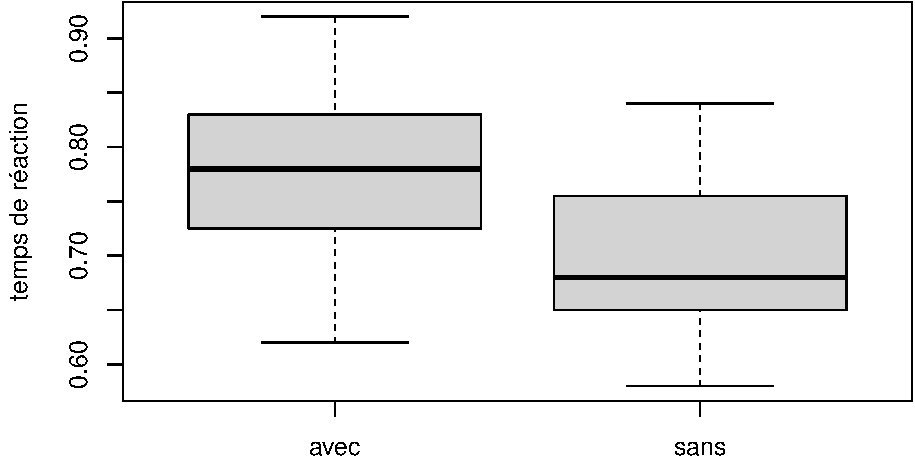
\includegraphics{sim1_td4_correction_files/figure-latex/unnamed-chunk-4-1.pdf}

Remarquons que le comportement n'est pas du tout le même chez les hommes
et chez les femmes. Le genre semble donc avoir un effet sur le lien
entre les variables ``temps'' et ``période''. C'est ce que l'on appelle
un \{\bf effet d'intéraction entre les deux facteurs\} de notre ANOVA.
Ainsi, dans une ANOVA à plusieurs facteurs, il est donc important de
prendre en compte les effets d'intéractions entre les différents
facteurs. Ce que l'on fait de la façon suivante :

\begin{Shaded}
\begin{Highlighting}[]
\NormalTok{res}\OtherTok{=}\FunctionTok{aov}\NormalTok{(temps}\SpecialCharTok{\textasciitilde{}}\NormalTok{sexe}\SpecialCharTok{+}\NormalTok{periode}\SpecialCharTok{+}\NormalTok{sexe}\SpecialCharTok{*}\NormalTok{periode,}\AttributeTok{data=}\NormalTok{data) }
\FunctionTok{print}\NormalTok{(}\FunctionTok{anova}\NormalTok{(res))}
\end{Highlighting}
\end{Shaded}

\begin{verbatim}
## Analysis of Variance Table
## 
## Response: temps
##              Df  Sum Sq Mean Sq F value    Pr(>F)    
## sexe          1  1372.7  1372.7  4.1502   0.04457 *  
## periode       4 19488.4  4872.1 14.7305 2.704e-09 ***
## sexe:periode  4 28085.0  7021.3 21.2284 2.359e-12 ***
## Residuals    90 29767.3   330.7                      
## ---
## Signif. codes:  0 '***' 0.001 '**' 0.01 '*' 0.05 '.' 0.1 ' ' 1
\end{verbatim}

On constate que cette interaction est en effet significative.

Il reste tout de même une chose à vérifier \ldots{} avons-nous le droit
de faire cette ANOVA ? Est-ce que toutes les conditions sont réunies ?\\

\begin{itemize}
\item[•] Ici, en ANOVA à 2 facteurs, il doit être grand ou gaussien pour chaque croisement de niveaux des 2 facteurs (période A - homme, période A - femme, . . . ). Donc clairement ici les échantillons ne sont pas grands. Il faut vérifier la normalité. Mais c’est impossible à faire pour chaque croisement de niveaux des facteurs, les données ne sont pas assez nombreuses et le test de Shapiro alors pas assez puissant. On se contente donc généralement en ANOVA à 2 facteurs de vérifier la normalité des résidus de
lVA\item[•] des variances homogènes pour chaque facteur.
\end{itemize}

Commençons par regarder la normalité des résidus.

\begin{Shaded}
\begin{Highlighting}[]
\FunctionTok{qqnorm}\NormalTok{(res}\SpecialCharTok{$}\NormalTok{residuals)}
\FunctionTok{qqline}\NormalTok{(res}\SpecialCharTok{$}\NormalTok{residuals)}
\end{Highlighting}
\end{Shaded}

\includegraphics{sim1_td4_correction_files/figure-latex/unnamed-chunk-6-1.pdf}

\begin{Shaded}
\begin{Highlighting}[]
\FunctionTok{shapiro.test}\NormalTok{(res}\SpecialCharTok{$}\NormalTok{residuals)}
\end{Highlighting}
\end{Shaded}

\begin{verbatim}
## 
##  Shapiro-Wilk normality test
## 
## data:  res$residuals
## W = 0.98482, p-value = 0.3081
\end{verbatim}

On peut accepter cette hypothèse de normalité des données car la p-value
est supérieure au risque de première espèce \(\alpha=0.05\).

Quant à l'homogénéité des variances, on peut la tester avec un test de
Bartlett, facteur par facteur.

\begin{Shaded}
\begin{Highlighting}[]
\FunctionTok{bartlett.test}\NormalTok{(temps}\SpecialCharTok{\textasciitilde{}}\NormalTok{periode,}\AttributeTok{data=}\NormalTok{data)}
\end{Highlighting}
\end{Shaded}

\begin{verbatim}
## 
##  Bartlett test of homogeneity of variances
## 
## data:  temps by periode
## Bartlett's K-squared = 19.856, df = 4, p-value = 0.0005331
\end{verbatim}

\begin{Shaded}
\begin{Highlighting}[]
\FunctionTok{bartlett.test}\NormalTok{(temps}\SpecialCharTok{\textasciitilde{}}\NormalTok{sexe,}\AttributeTok{data=}\NormalTok{data)}
\end{Highlighting}
\end{Shaded}

\begin{verbatim}
## 
##  Bartlett test of homogeneity of variances
## 
## data:  temps by sexe
## Bartlett's K-squared = 6.239, df = 1, p-value = 0.0125
\end{verbatim}

L'homogénéite des variances n'est pas respectée ici. En effet, la
p-value est ici bien inférieure à \(0.05\) pour les deux facteurs.
Néanmoins l'ANOVA reste assez robuste à la non homogénéite des variances
lorsque les effectifs ne sont pas trop différents d'une modalité à
l'autre, ce qui est le cas ici. De plus, il n'existe pas d'alternative
non paramétrique à l'ANOVA à 2 facteurs. (Pour l'ANOVA à 1 facteur, on
aurait pu passer à un test de Kruskall).\\

On peut regarder le graphique ci-dessous qui nous montre comment évolue
les différentes moyennes en fonction des différents facteurs.

\begin{Shaded}
\begin{Highlighting}[]
\FunctionTok{interaction.plot}\NormalTok{(data}\SpecialCharTok{$}\NormalTok{sexe,data}\SpecialCharTok{$}\NormalTok{periode,data}\SpecialCharTok{$}\NormalTok{temps)}
\end{Highlighting}
\end{Shaded}

\includegraphics{sim1_td4_correction_files/figure-latex/unnamed-chunk-8-1.pdf}

On peut aussi aller plus en détail pour faire des tests deux à deux
entre modalité, au niveau des périodes. Pour contrecarer les
problématiques de multiplicité des tests, on utilise des corrections
comme celle de Bonferroni:

\begin{Shaded}
\begin{Highlighting}[]
\FunctionTok{pairwise.t.test}\NormalTok{(data}\SpecialCharTok{$}\NormalTok{temps,data}\SpecialCharTok{$}\NormalTok{periode,}\AttributeTok{p.adjust.method =} \StringTok{"bonferroni"}\NormalTok{)}
\end{Highlighting}
\end{Shaded}

\begin{verbatim}
## 
##  Pairwise comparisons using t tests with pooled SD 
## 
## data:  data$temps and data$periode 
## 
##   A      B      C       D     
## B 1.0000 -      -       -     
## C 0.3731 0.0066 -       -     
## D 1.0000 1.0000 0.2837  -     
## E 0.0158 0.6834 5.7e-06 0.0225
## 
## P value adjustment method: bonferroni
\end{verbatim}

Ici on remarque par exemple que les périodes \(B\) et \(C\) sont
significativement différentes alors que \(A\) et \(C\) ne le sont pas.

\hypertarget{exercice-2}{%
\subsection{Exercice 2}\label{exercice-2}}

On se propose de travailler à nouveau sur le fichier GermanCredit afin
de répondre à plusieurs questions. Cet exercice est très proche de ce
qui vous attendra à l'examen.

\hypertarget{question-1}{%
\subsubsection{Question 1}\label{question-1}}

On cherche à savoir si le sexe (variable quali) à une influence sur le
montant emprunté (variable quanti) et plus précisément si les femmes
empruntent un montant plus important que les hommes. On formule alors
les hypothèses suivantes :

\begin{itemize}
\item[•] $H_0 :$ 
\item[•] $H_1 :$ 
\end{itemize}

\hypertarget{question-2}{%
\subsubsection{Question 2}\label{question-2}}

On cherche à savoir si l'emploi (variable quali) et le sexe (variable
quali) ont une influence sur la durée de l'emprunt (variable quanti). On
formule alors les hypothèses suivantes :

\begin{itemize}
\item[•] $H_0 :$ 
\item[•] $H_1 :$ 
\end{itemize}

\hypertarget{question-3}{%
\subsubsection{Question 3}\label{question-3}}

On se propose ensuite d'étudier si les variables ``montant du crédit''
(variable quanti) et ``durée de l'emprunt'' (variable quanti) sont des
variables gaussiennes. On formule alors les hypothèses suivantes :

\begin{itemize}
\item[•] $H_0 :$ 
\item[•] $H_1 :$ 
\end{itemize}

\hypertarget{question-4}{%
\subsubsection{Question 4}\label{question-4}}

On cherche à savoir si le montant du crédit (variable quanti) est lié au
but du crédit (variable quali). On formule alors les hypothèses
suivantes :

\begin{itemize}
\item[•] $H_0 :$ 
\item[•] $H_1 :$ 
\end{itemize}

\hypertarget{question-5}{%
\subsubsection{Question 5}\label{question-5}}

On cherche à savoir si le montant emprunté est différent selon notre
situation personnelle en terme de logement (propriétaire, locataire,
\ldots). On formule alors les hypothèses suivantes :

\begin{itemize}
\item[•] $H_0 :$ 
\item[•] $H_1 :$ 
\end{itemize}

\hypertarget{question-6}{%
\subsubsection{Question 6}\label{question-6}}

Enfin, on souhaite savoir si le montant du crédit est lié à la durée de
ce dernier. On formule alors les hypothèses suivantes :

\begin{itemize}
\item[•] $H_0 :$ 
\item[•] $H_1 :$ 
\end{itemize}

\end{document}
